\section{Coexistence Scenarios}

The previous section investigated the borders where stable cycles disappear.
We can see that parameter regions where only one stable cycle exists (``Type A'') can overlap.
For example, the upper border where the cycle $\Cycle{\A^5\B^3\C^5\D^3}$ disappears, marked blue in \Cref{fig:final.regions.E.halved}, is above the lower border where the stable cycle $\Cycle{\A^4\B^3\C^4\D^3}$ disappears, marked red.
This means that there is a coexistence of the cycles in the overlapping parameter region, marked with the point $M$.
This section will take a look at all possible coexistence scenarios of cycles starting with the simplest case, a single ``Type A'' parameter region.

\begin{figure}
    \centering
    \begin{subfigure}{0.4\textwidth}
        \centering
        \includegraphics[width=\textwidth]{60_MinimalRepr/2D_Regions_E/result.png}
        \caption{Showing $E_{16}$}
        \label{fig:final.regions.E.halved}
    \end{subfigure}
    \begin{subfigure}{0.4\textwidth}
        \centering
        \includegraphics[width=\textwidth]{60_MinimalRepr/2D_Regions_F/result.png}
        \caption{Showing $F_{16}$}
        \label{fig:final.regions.F.halved}
    \end{subfigure}
    \caption{2D Period Regions of Halved Final Model Showing a ``Type A'' and a ``Type B'' Region}
\end{figure}
